\documentclass[12pt]{article}

\usepackage[utf8]{inputenc}
\usepackage[english,russian]{babel}
\usepackage[left=2cm,right=2cm,top=2cm,bottom=2cm,bindingoffset=0cm]{geometry}
\usepackage{indentfirst}
\usepackage{comment}
\usepackage{pythonhighlight}
\usepackage{amssymb}
\usepackage{graphicx}
\usepackage{float}
\usepackage{wrapfig}


\usepackage[colorlinks, linkcolor = blue]{hyperref}


\newtheorem{sttm}{Утверждение}
\newtheorem{hyp}{Гипотеза}
\newtheorem{offer}{Предложение}

\newcommand{\qed}{\hfill $\blacksquare$}

\everymath{\displaystyle}



\begin{document}
	\title{Применение MDL (Minimal Descripton length) принципа Риссанена для марковских процессов.}
	\author{Ремизова Анна Петровна}
	\maketitle
	
	\section*{Что нового}
	\begin{enumerate}
		\item Доказательство Утверждения~(\ref{sttm:independence}), котрое обсудили при встрече, немного скорректировала формулировку: вместо "берутся первые k и l знаков p и q" - "при заданных длинах двоичной записи $k$ и $l$ - это приближения оптимальных значений $p$ и $q$ числами вида $x=\frac{n}{2^{k}}$ и $x=\frac{n}{2^{l}}$ соответственно", добавила Рис.~(\ref{pic:P(x,p)}) с графиками.
		\item Исправила и пояснила выводы по таблицам с учётом посчитанных по формулам оптимальных $p$ и $q$ (то, что написала в сообщении).
		\item Начала главу про Марковские цепи с 4 состояниями, но пока не сделала моделирование и перебор.
	\end{enumerate}
	
	\section*{Введение}
	 Есть данные, мы хотим подобрать марковскую цепь, для которой наибольшая вероятность получить заданную траекторию. По Риссанену, если мы хотим предсказать, что будет дальше, то должны сравнивать друг с другом гипотезы по их сложности, причём даём преимущество простым гипотезам. Выражения для Description length будет выглядеть следующим образом:
	
	\begin{equation}C(\mu)+\log_2{\frac{1}{\mu(x)}}\end{equation}
	
	где $C(\mu)$ -- complexity, $\mu$ -- распределение вероятности.
	
	\section*{Марковские цепи с 2 состояниями}
	Для начала рассмотрим простые марковские цепи. Пусть марковская цепь состоит из 2 состояний. Дана последовательность состояний Марковской цепи из 2 состояний: 0 и 1. Найти оптимальные переходные вероятности $p$ из 0 в 1 и $q$ из 1 в 0 по принципу Риссанена MDL. 
	
	Для решения этой задачи запишем вероятность получения заданной реализации: пусть $n(ij)$ -- число переходов из состояния $i$ в состояние $j$, тогда:
	
	\begin{equation}P_c(x) = p^{n(01)}\cdot(1-p)^{n(00)}\cdot q^{n(10)}\cdot(1-q)^{n(11)}\to max\end{equation}
	
	\begin{equation}\label{log}\log_2{\frac{1}{P_c(x)}}=-(n(01)\cdot\log_2{p}+n(00)\cdot\log_2{(1-p)}+n(10)\cdot\log_2{q}+n(11)\cdot\log_2{(1-q)})\end{equation}
	
	Сложность $C(\mu)$ будем определять как суммарную длину записи $p$ и $q$ в двоичной системе счисления. Пусть вероятность $p$ имеет $k$ знаков в двоичной системе, $q$ -- $l$ знаков, тогда $C(\mu)=k+l$. Далее рассмотрим несколько реализаций Марковских цепей и исследуем, как меняются значения в зависимости от $k$ и $l$.
	
	\subsection*{Таблица с двоичными значениями}
	В Таблицах~(\ref{table:piBinary},~\ref{table:2Binary},~\ref{table:3Binary}) в каждой ячейке представлены сначала оптимальные (минимальные, т.к. ищем минимальную описательную длину) значения $\log_2{\frac{1}{\mu(x)}}=-(n_{01}\log_2{p}+n_{00}\log_2{(1-p)}+n_{10}\log_2{q}+n_{11}\log_2{(1-q)})$, затем сложность по Риссанену, а после - значения $p$ и $q$, при которых оно достигается, представленные в двоичной системе счисления, для марковских цепей с траекториями, соответствующими 30 первым знакам $\pi, sqrt(2), sqrt(3)$ соответственно. По горизонтали отмечены значения $l$ - длина перебираемых $q$  в двоичной системе, по вертикали - значения $k$ - длина перебираемых $p$  в двоичной системе.
	
	
	\begin{table}[h]
		\caption{Таблица оптимальных зн-й p и q в двоичной записи для $\pi$}
		\label{table:piBinary}
		\begin{center}
			\begin{tabular}{|l|l|l|l|l|l|l|}
				\hline
				k / l &1 & 2 & 3 & 4 & 5 & 6\\
				\hline
				1 & 31.0& 32.0& 33.0& 33.9891& 34.9521& 35.9521\\
				& 29.0& 29.0& 29.0& 28.9891& 28.9521& 28.9521\\
				& 0.1& 0.1& 0.1& 0.1& 0.1& 0.1\\
				& 0.1& 0.10& 0.100& 0.1001& 0.10001& 0.100010\\
				\hline
				2 & 32.0& 33.0& 34.0& 34.9891& 35.9521& 36.9521\\
				& 29.0& 29.0& 29.0& 28.9891& 28.9521& 28.9521\\
				& 0.10& 0.10& 0.10& 0.10& 0.10& 0.10\\
				& 0.1& 0.10& 0.100& 0.1001& 0.10001& 0.100010\\
				\hline
				3 & 33.0& 34.0& 35.0& 35.9891& 36.9521& 37.9521\\
				& 29.0& 29.0& 29.0& 28.9891& 28.9521& 28.9521\\
				& 0.100& 0.100& 0.100& 0.100& 0.100& 0.100\\
				& 0.1& 0.10& 0.100& 0.1001& 0.10001& 0.100010\\
				\hline
				4 & 34.0& 35.0& 36.0& 36.9891& 37.9521& 38.9521\\
				& 29.0& 29.0& 29.0& 28.9891& 28.9521& 28.9521\\
				& 0.1000& 0.1000& 0.1000& 0.1000& 0.1000& 0.1000\\
				& 0.1& 0.10& 0.100& 0.1001& 0.10001& 0.100010\\
				\hline
				5 & 35.0& 36.0& 37.0& 37.9891& 38.9521& 39.9521\\
				& 29.0& 29.0& 29.0& 28.9891& 28.9521& 28.9521\\
				& 0.10000& 0.10000& 0.10000& 0.10000& 0.10000& 0.10000\\
				& 0.1& 0.10& 0.100& 0.1001& 0.10001& 0.100010\\
				\hline
				6 & 36.0& 37.0& 38.0& 38.9891& 39.9521& 40.9521\\
				& 29.0& 29.0& 29.0& 28.9891& 28.9521& 28.9521\\
				& 0.100000& 0.100000& 0.100000& 0.100000& 0.100000& 0.100000\\
				& 0.1& 0.10& 0.100& 0.1001& 0.10001& 0.100010\\
				\hline
			\end{tabular}
		\end{center}
	\end{table}
	
	
	Выводы к Таблице~(\ref{table:piBinary}) для $\pi$: заметим, что при фиксированной длине l (по столбцам) двоичной записи переходной вероятности q оптимальное значение q неизменно, но при этом с увеличением k оптимальное значение логарифма уменьшается. Аналогично для фиксированного k (по строкам).
	
	\begin{table}[h]
		\caption{Таблица оптимальных зн-й p и q в двоичной записи для $\sqrt{2}$}
		\label{table:2Binary}
		\begin{center}
			\begin{tabular}{|l|l|l|l|l|l|l|}
				\hline
				k / l &1 & 2 & 3 & 4 & 5 & 6\\
				\hline
				1 & 31.0& 32.0& 32.9148& 33.7965& 34.7965& 35.795\\
				& 29.0& 29.0& 28.9148& 28.7965& 28.7965& 28.795\\
				& 0.1& 0.1& 0.1& 0.1& 0.1& 0.1\\
				& 0.1& 0.10& 0.101& 0.1001& 0.10010& 0.100101\\
				\hline
				2 & 32.0& 33.0& 33.9148& 34.7965& 35.7965& 36.795\\
				& 29.0& 29.0& 28.9148& 28.7965& 28.7965& 28.795\\
				& 0.10& 0.10& 0.10& 0.10& 0.10& 0.10\\
				& 0.1& 0.10& 0.101& 0.1001& 0.10010& 0.100101\\
				\hline
				3 & 33.0& 34.0& 34.9148& 35.7965& 36.7965& 37.795\\
				& 29.0& 29.0& 28.9148& 28.7965& 28.7965& 28.795\\
				& 0.100& 0.100& 0.100& 0.100& 0.100& 0.100\\
				& 0.1& 0.10& 0.101& 0.1001& 0.10010& 0.100101\\
				\hline
				4 & 33.9891& 34.9891& 35.9039& 36.7856& 37.7856& 38.7842\\
				& 28.9891& 28.9891& 28.9039& 28.7856& 28.7856& 28.7842\\
				& 0.0111& 0.0111& 0.0111& 0.0111& 0.0111& 0.0111\\
				& 0.1& 0.10& 0.101& 0.1001& 0.10010& 0.100101\\
				\hline
				5 & 34.9521& 35.9521& 36.8669& 37.7485& 38.7485& 39.7471\\
				& 28.9521& 28.9521& 28.8669& 28.7485& 28.7485& 28.7471\\
				& 0.01111& 0.01111& 0.01111& 0.01111& 0.01111& 0.01111\\
				& 0.1& 0.10& 0.101& 0.1001& 0.10010& 0.100101\\
				\hline
				6 & 35.9521& 36.9521& 37.8669& 38.7485& 39.7485& 40.7471\\
				& 28.9521& 28.9521& 28.8669& 28.7485& 28.7485& 28.7471\\
				& 0.011110& 0.011110& 0.011110& 0.011110& 0.011110& 0.011110\\
				& 0.1& 0.10& 0.101& 0.1001& 0.10010& 0.100101\\
				\hline
			\end{tabular}
		\end{center}
	\end{table}
	
	Выводы к Таблице~(\ref{table:2Binary}): для $\sqrt{2}$ практически то же, что и для $\pi$.
	
	\begin{table}[h]
		\caption{Таблица оптимальных зн-й p и q в двоичной записи для $\sqrt{3}$}
		\label{table:3Binary}
		\begin{center}
			\begin{tabular}{|l|l|l|l|l|l|l|}
				\hline
				k / l &1 & 2 & 3 & 4 & 5 & 6\\
				\hline
				1 & 31.0& 32.0& 33.0& 33.8419& 34.8419& 35.8419\\
				& 29.0& 29.0& 29.0& 28.8419& 28.8419& 28.8419\\
				& 0.1& 0.1& 0.1& 0.1& 0.1& 0.1\\
				& 0.1& 0.10& 0.100& 0.0111& 0.01110& 0.011100\\
				\hline
				2 & 31.9053& 32.9053& 33.9053& 34.7472& 35.7472& 36.7472\\
				& 28.9053& 28.9053& 28.9053& 28.7472& 28.7472& 28.7472\\
				& 0.11& 0.11& 0.11& 0.11& 0.11& 0.11\\
				& 0.1& 0.10& 0.100& 0.0111& 0.01110& 0.011100\\
				\hline
				3 & 32.4067& 33.4067& 34.4067& 35.2486& 36.2486& 37.2486\\
				& 28.4067& 28.4067& 28.4067& 28.2486& 28.2486& 28.2486\\
				& 0.101& 0.101& 0.101& 0.101& 0.101& 0.101\\
				& 0.1& 0.10& 0.100& 0.0111& 0.01110& 0.011100\\
				\hline
				4 & 33.4067& 34.4067& 35.4067& 36.2486& 37.2486& 38.2486\\
				& 28.4067& 28.4067& 28.4067& 28.2486& 28.2486& 28.2486\\
				& 0.1010& 0.1010& 0.1010& 0.1010& 0.1010& 0.1010\\
				& 0.1& 0.10& 0.100& 0.0111& 0.01110& 0.011100\\
				\hline
				5 & 34.4067& 35.4067& 36.4067& 37.2486& 38.2486& 39.2486\\
				& 28.4067& 28.4067& 28.4067& 28.2486& 28.2486& 28.2486\\
				& 0.10100& 0.10100& 0.10100& 0.10100& 0.10100& 0.10100\\
				& 0.1& 0.10& 0.100& 0.0111& 0.01110& 0.011100\\
				\hline
				6 & 35.4029& 36.4029& 37.4029& 38.2448& 39.2448& 40.2448\\
				& 28.4029& 28.4029& 28.4029& 28.2448& 28.2448& 28.2448\\
				& 0.101001& 0.101001& 0.101001& 0.101001& 0.101001& 0.101001\\
				& 0.1& 0.10& 0.100& 0.0111& 0.01110& 0.011100\\
				\hline
			\end{tabular}
		\end{center}
	\end{table}
	
	Выводы к Таблице~(\ref{table:3Binary}): для $\sqrt{3}$ результаты уже отличаются от $\pi$, но наблюдаются те же закономерности. Отличие $\sqrt{3}$ от $\pi$ и $\sqrt{2}$ в количестве диграмм в их двоичной записи, были рассмотрены первые 30 знаков для каждого числа, не считая точки. Если для $\pi$ и $\sqrt{2}$ распределение количества диграмм близко к равномерному, то для $\sqrt{3}$ оно менее сбалансированно: количество диграмм 00 меньше остальных, а диграмм 11 - больше (см.Таблицу~\ref{table:digramsPi23}).
	
	\begin{sttm}\label{sttm:independence} Оптимальное значение p не зависит от q и наоборот, оптимальное значение q не зависит от p.
	\end{sttm}
	{\bf Доказательство.} Рассмотрим выражение (\ref{log}) для логарифма. Значения $n(00), n(01), n(10), n(11)$ -- постоянные, и данное выражения можно представить в виде линейной комбинации двух функций $f_1(p)+f_2(q)$. Соотвественно, при максимизации всего выражения (логарифм (\ref{log}) должен быть маленьким, а так как перед всем выражением стоит минус, то выражение в скобках должно быть большим), так как переменные $p$ и $q$ содержатся в отдельных слагаемых, необходимо найти минимум отдельно для $f_1(p)$ и $f_2(q)$, друг на друга их значения при минимизации не влияют. \qed
	
	\subsection*{Анализ диграмм}
	В Таблице~(\ref{table:digramsPi23}) представлены количества диграмм по рассмотренным примерам - их сумма в каждом случае равна 29, так как рассматриваемые числа округлялись до 30 знаков в двоичной записи суммарно, далее оптимальные значения $k,l,\log_2{\frac{1}{\mu{x}}},MDL$, найденные при $k,l\in[1,6]$ для минимизации $MDL$.
	\begin{sttm}\label{derivative}Значения $p = \frac{n(01)}{n(01)+n(00))}$ и $q = \frac{n(10)}{n(10)+n(11)}$ являются точкой максимума функции $\log_2{\frac{1}{P_c(x)}}$~(\ref{log}). Их значения при заданных длинах двоичной записи $k$ и $l$ - это приближения оптимальных значений $p$ и $q$ числами вида $x=\frac{n}{2^{k}}$ и $x=\frac{n}{2^{l}}$ соответственно.\end{sttm}
	{\bf Доказательство}
	\begin{enumerate}
	\item Найдём точку максимума функции $f_1(p) = n(01)\log_2{p} + n(00)\log_2{(1-p)}$. Её производная: $f'_1(p) = \frac{n(01)}{p\ln{2}} - \frac{n(00)}{(1-p)\ln{2}}$, критические точки $p=\frac{n(01)}{n(01)+n(00)},p=0,p=1$. Т.к. $0\le\frac{n(01)}{n(01)+n(00)}\le1$, то $f'_1(p)$ отрицательна на $p\in(-\infty;0)\cup\left(\frac{n(01)}{n(01)+n(00)};1\right)$, положительная на остальных промежутках, а значит точка максимума $p = \frac{n(01)}{n(01)+n(00)}$, если это значение отлично от $0$ и $1$, и $p=0$ иначе. Аналогично для $f_2(q)$ точкой максимума является $q=\frac{n(10)}{n(10)+n(11)}$, либо $q=0$.
	
	\item Рассмотрим функцию вероятности $P(x) = x^p(1-x)^{1-p}$. Найдём её вторую производную: $P'(x) = (1-x)^{-p} (p-x) x^{p-1}, P''(x)=(p-1) p (1-x)^{-p-1} x^{p-2}$. При фиксированном p $P''(x)$ имеет нули в точках $x=0, x=1$ и $P''(x)\ge0$ на $x\in[0;1]$, а значит на этом интервале исходная функция выпукла вверх -- см. Рис.~(\ref{pic:P(x,p)}). Кроме того, её максимальное значение достигается при $x=p$. Так как при фиксированном $k$ мы рассматриваем двоичные числа с $k$ знаками после запятой, то $x=\frac{n}{2^{k}}$. Соответственно, оптимальным будет именно приближение точки максимума функции $P(x): x = p$, а будет это приближение с избытком или недостатком -- зависит от того, какое из чисел будет ближе к $p$ по значению функции $P(x)$.
	
	\begin{figure}[h]
		\label{pic:P(x,p)}
		\centering
		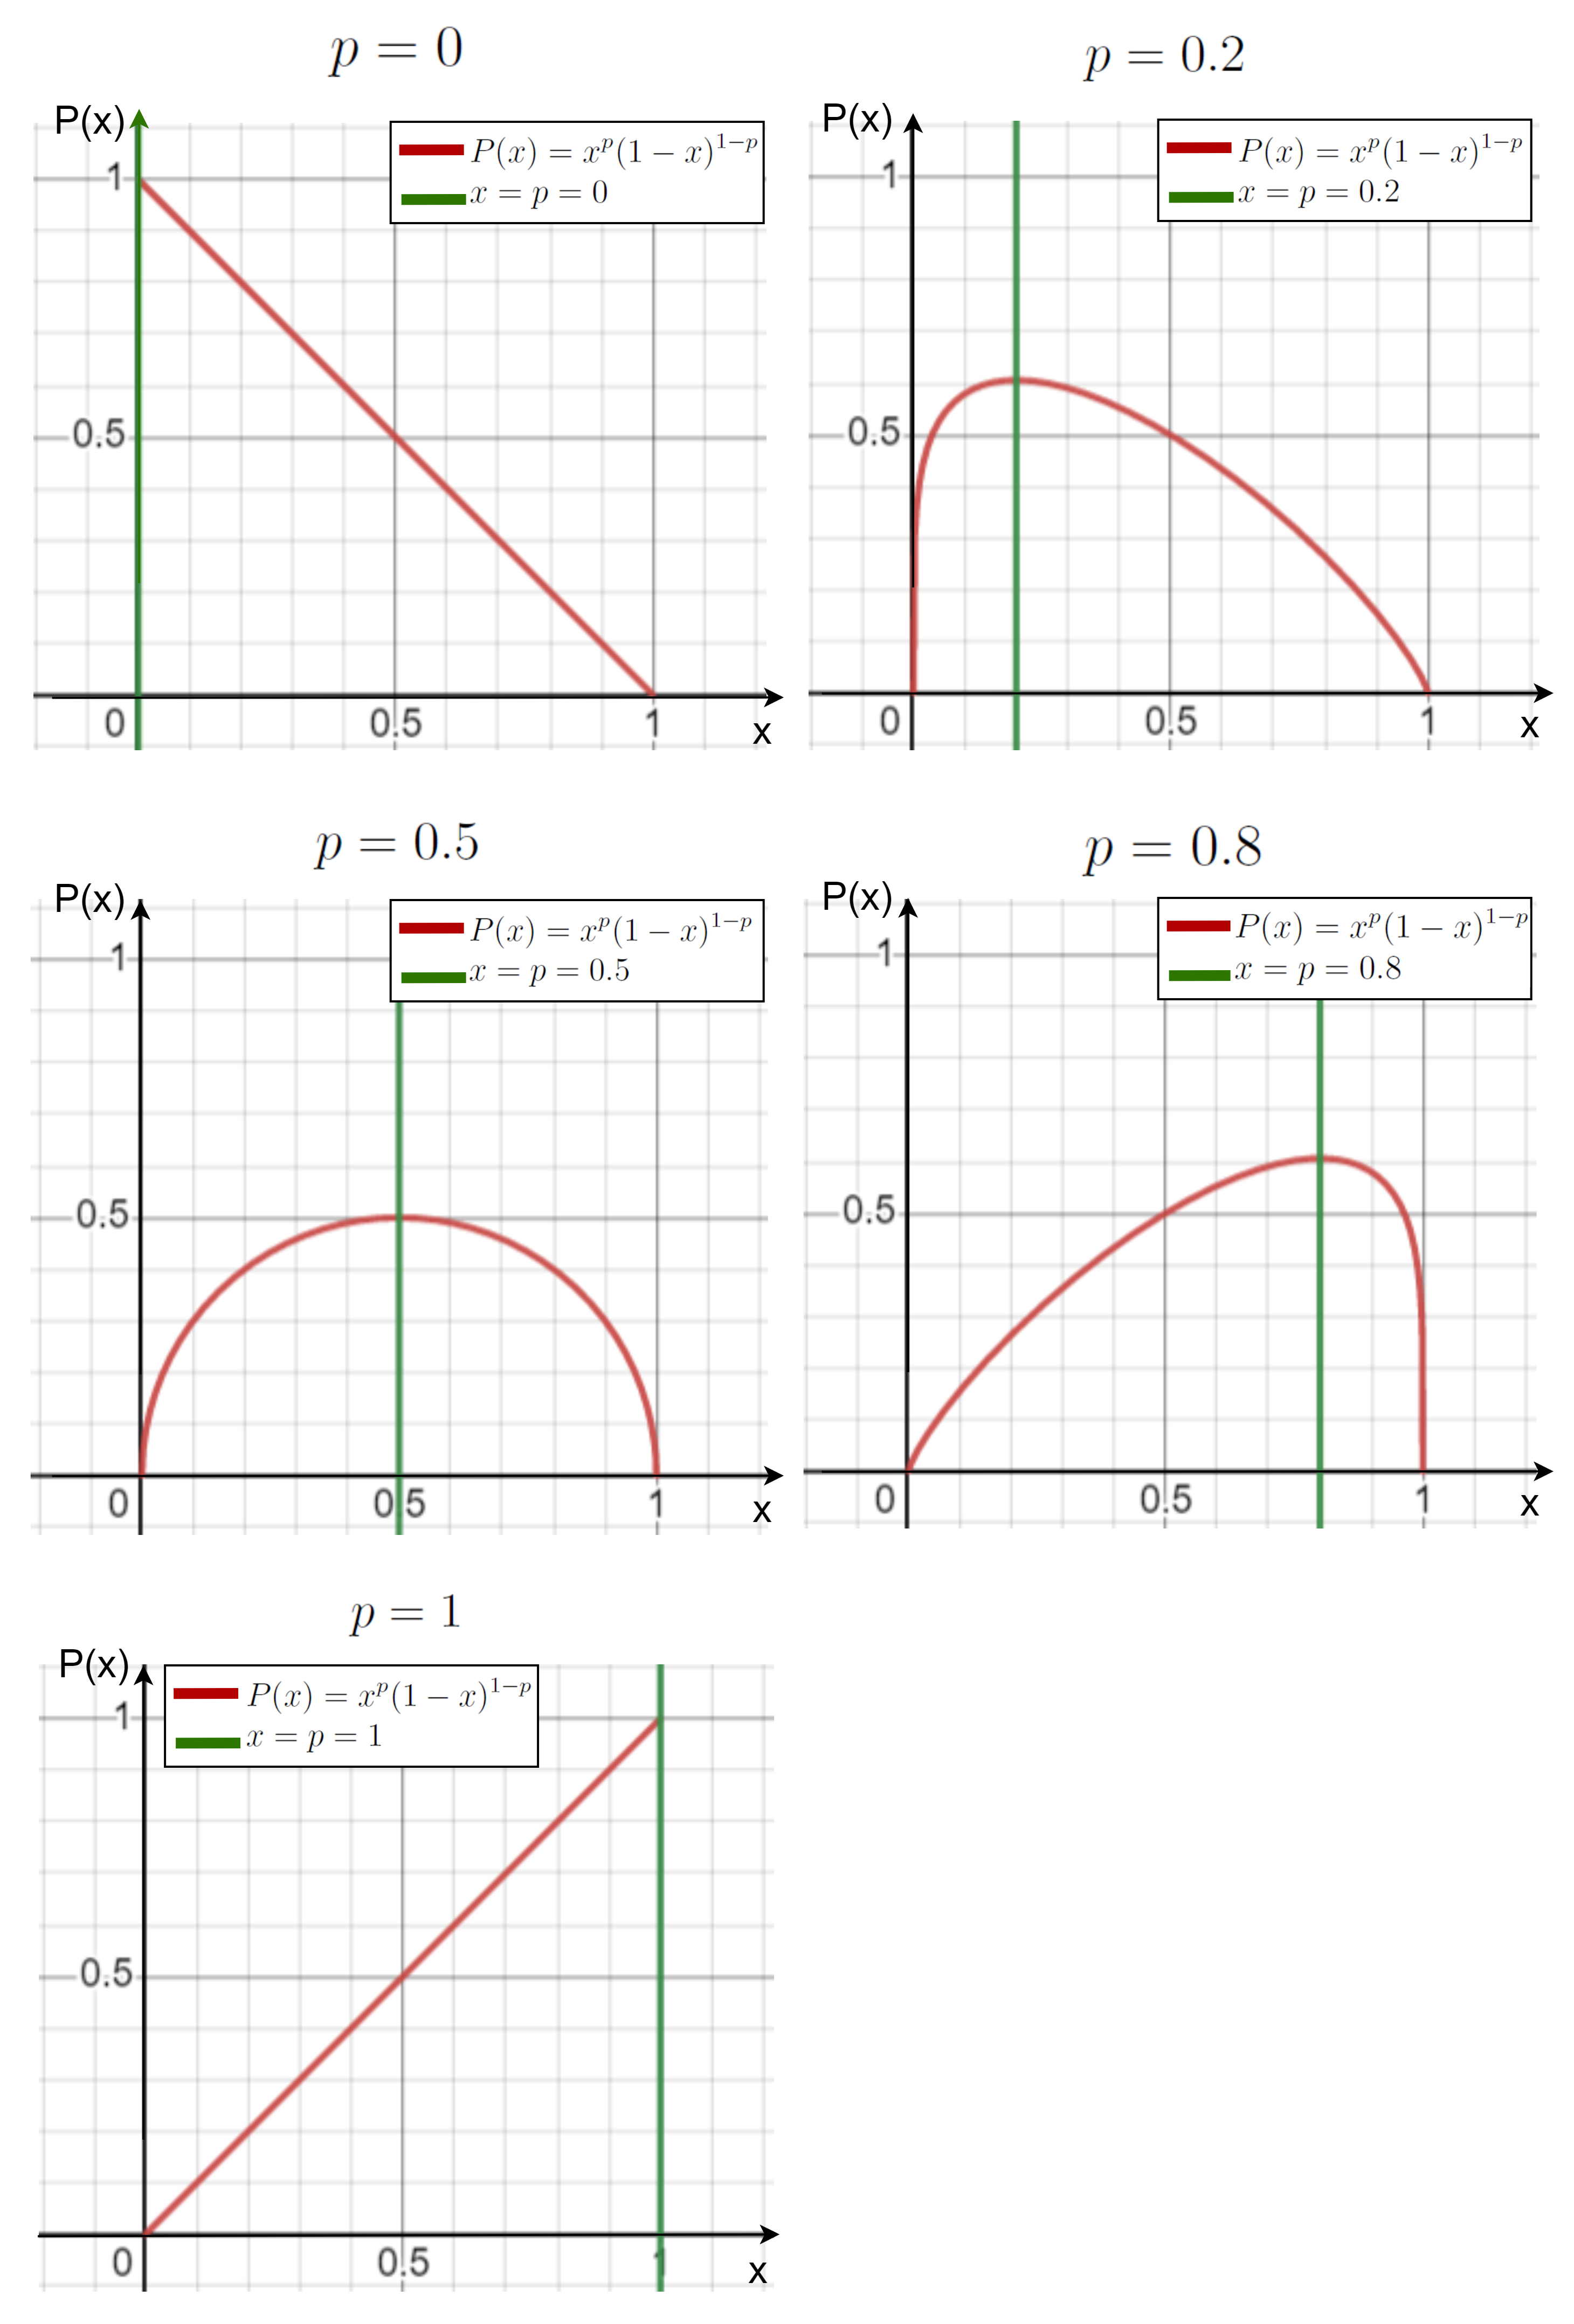
\includegraphics[width=0.8\linewidth]{images/p(x,p).png}
		\caption{График функции $P(x)$ при различных значениях $p$}
	\end{figure}
	
	
	
	\item Для $\pi$ оптимальные $p$ и $q$, вычисленные по указанным формулам, выглядят следующим образом: $p_0=0.5_{10} = 0.1_2, q_0=0.5(3)_{10}=0.(1000)_2$, чему удовлетворяют значения из Таблицы~(\ref{table:piBinary}). 
	
	Для $\sqrt{2}$ имеем: $p_0=0.4(6)_{10}=0.(0111)_2, q_0=0.(571428)_{10}=0.(100)_2$ -- по Таблице~(\ref{table:2Binary}) совпадает $q$, но не совпадает, на первый взгляд, $p$. Но значение, представленное в таблице, к примеру, для $k=6$ -- это $0.011110_2 = \frac{30}{64}_{10}$, а значение, равное округлению до 6 знаков после запятой найденного по формуле $p$ -- это $0.011101_2 = \frac{29}{64}_{10}$ И действительно, если обозначить $p_0$ - найденное по формуле, то $\frac{29}{64} < p_0 < \frac{30}{64}$ и $0.00019\approx\left|f_1(p_0)-f_1\left(\frac{30}{64}\right)\right| < \left|f_1(p_0)-f_1\left(\frac{29}{64}\right)\right|\approx0.00800$.
	
	Для $\sqrt{3}$ имеем: $p_0=0.(63)_{10}=0.(1010001011)_2, q_0=0.(4)_{10}=0.(011100)_2$ -- по Таблице~(\ref{table:3Binary}) также совпадает $q$, и также совпадает $p$ с верхним приближением: для $k=6$, к примеру, $0.101001_2 = \frac{41}{64}_{10},\;0.101000_2 = \frac{40}{64}_{10},\;\frac{40}{64}<p_0<\frac{41}{64}$. 
	
	Таким образом, на представленных примерах всё согласуется с утверждением.\qed
	\end{enumerate}
	
	\begin{table}[!h]
		\caption{Числа, количество диграмм в них, оптимальные k и l}
		\label{table:digramsPi23}
		\begin{center}
			\begin{tabular}{|l|l|l|l|l|l|l|l|l|}
			\hline
			Число & $n(00)$ & $n(01)$ & $n(10)$ & $n(11)$ & k & l & $\log_2{\frac{1}{\mu(x)}}$& MDL\\
			\hline
			$\pi$ & 7 & 7 & 8 & 7 & 1 & 1 & 29.0 & 31.0\\
			\hline
			$\sqrt{2}$ & 8 & 7 & 8 & 6 & 1 & 1 & 29.0 & 31.0\\
			\hline
			$\sqrt{3}$ & 4 & 7 & 8 & 10 & 1 & 1 & 29.0 & 31.0\\
			\hline
		\end{tabular}
	\end{center}
	\end{table}

	Заметим по Таблице~(\ref{table:digramsPi23}), что для рассмотренных трёх случаев высокая точность переходных вероятностей $p$ и $q$ не выгодна по Риссанену, Minimal description length достигается при $k=l=1$. Это будет не так, если при увеличении на 1 бит точности переходной вероятности логарифм будет уменьшаться больше, чем на 1. Т.е. количество диграмм $n(00)$ и $n(01)$ должно быть сильно не сбалансированно. % вот это мне не до конца понятно, почему
	
	Рассмотрим различные значения $n(01)$ для $n(00)=1$ и найдём, при каком k достигается MDL. Алгоритм: берём $p = \frac{n(01)}{n(01)+n(00))}$, переводим в двоичнyю систему с k знаками после запятой, считаем для каждого $Description length = k - (n(01)\log_2{p}+n(00)\log_2{(1-p)})$ и ищем минимальное такое при различных $k\in[1,100]$ В Таблице~(\ref{table:n00n01}) видно, что результаты $k$ уже нетривиальные -- мы нашли те примеры последовательностей, для которых оптимальная модель подразумевает достаточно точные значения переходных вероятностей. Симметричная ситуация будет наблюдаться и для $l$.
	
	\begin{table}[!h]
		\caption{Оптимальные k для разных n(01)}
		\label{table:n00n01}
		\begin{center}
			\begin{tabular}{|l|l|l|l|l|}
				\hline
				n(00) & n(01) & k & p & MDL \\
				\hline
				1 & 2 & 1 & 0.1 & 4.0 \\ 
				\hline 
				1 & 4 & 2 & 0.11 & 5.6601 \\ 
				\hline 
				1 & 8 & 2 & 0.11 & 7.3203 \\ 
				\hline 
				1 & 16 & 3 & 0.111 & 9.0823 \\ 
				\hline 
				1 & 32 & 4 & 0.1111 & 10.9795 \\ 
				\hline 
				1 & 64 & 5 & 0.11111 & 12.9314 \\ 
				\hline 
				1 & 128 & 6 & 0.111111 & 14.9082 \\ 
				\hline 
				1 & 256 & 7 & 0.1111111 & 16.8967 \\ 
				\hline 
				1 & 512 & 8 & 0.11111111 & 18.891 \\ 
				\hline 
				1 & 1024 & 9 & 0.111111111 & 20.8882 \\ 
				\hline 
			\end{tabular}
		\end{center}
	\end{table}

	\section*{Марковские цепи с 4 состояниями}
	Рассмотрим более сложную марковскую цепь с четырьмя состояниями, но по-прежнему над двоичным алфавитом. Пусть при посещении состояний $a, b$ печатаются нули, при посещении состояний $c, d$ -- единицы. Для некоторых последовательностей, в частности для тех, которые имеют период 4, например $00010001\dots0001$, такая модель будет давать более оптимальный с точки зрения MLD результат.
		
	
	\begin{comment} % подписи для рисунков
	$P(x) = x^p(1-x)^{1-p}$
	
	$x = p = 1$
	
	$p = 1$
	
	$p = 0$
	
	$P(x) = x^p(1-x)^{1-p}$
	
	$x = p = 0$
	
	$p = 0.2$
	
	$P(x) = x^p(1-x)^{1-p}$
	
	$x = p = 0.2$
	
	$p = 0.5$
	
	$P(x) = x^p(1-x)^{1-p}$
	
	$x = p = 0.5$
	
	$p = 0.8$
	
	$P(x) = x^p(1-x)^{1-p}$
	
	$x = p = 0.8$\end{comment}
	
	

	\begin{comment}	\subsection*{Таблица с десятичными значениями}
	В таблице в каждой ячейке представлены сначала оптимальные значения $C(\mu)+\log_2{\frac{1}{\mu(x)}}$, затем $p$ и $q$, при которых оно достигается, округлённые до десятитысячных. По горизонтали отмечены значения $l$ - длина перебираемых $q$  в двоичной системе, по вертикали - значения $k$ - длина перебираемых $p$  в двоичной системе.
	
	\begin{table}[h]
		\caption{Таблица оптимальных значений p и q для $\pi$}
		\label{table:piDecimal}
		\begin{center}
			\begin{tabular}{|l|l|l|l|l|l|l|}
				\hline
				k / l &1 & 2 & 3 & 4 & 5 & 6\\
				\hline
				1 & 0.5& 0.5& 0.5& 0.5& 0.5& 0.5\\
				& 0.5& 0.5& 0.625& 0.625& 0.625& 0.6094\\
				& 25.0& 25.0& 24.4998& 24.4998& 24.4998& 24.4975\\
				\hline
				2 & 0.5& 0.5& 0.5& 0.5& 0.5& 0.5\\
				& 0.5& 0.5& 0.625& 0.625& 0.625& 0.6094\\
				& 25.0& 25.0& 24.4998& 24.4998& 24.4998& 24.4975\\
				\hline
				3 & 0.625& 0.625& 0.625& 0.625& 0.625& 0.625\\
				& 0.5& 0.5& 0.625& 0.625& 0.625& 0.6094\\
				& 24.8217& 24.8217& 24.3215& 24.3215& 24.3215& 24.3192\\
				\hline
				4 & 0.5625& 0.5625& 0.5625& 0.5625& 0.5625& 0.5625\\
				& 0.5& 0.5& 0.625& 0.625& 0.625& 0.6094\\
				& 24.7738& 24.7738& 24.2735& 24.2735& 24.2735& 24.2713\\
				\hline
				5 & 0.5938& 0.5938& 0.5938& 0.5938& 0.5938& 0.5938\\
				& 0.5& 0.5& 0.625& 0.625& 0.625& 0.6094\\
				& 24.7623& 24.7623& 24.2621& 24.2621& 24.2621& 24.2598\\
				\hline
				6 & 0.5781& 0.5781& 0.5781& 0.5781& 0.5781& 0.5781\\
				& 0.5& 0.5& 0.625& 0.625& 0.625& 0.6094\\
				& 24.7594& 24.7594& 24.2592& 24.2592& 24.2592& 24.2569\\
				\hline
			\end{tabular}
		\end{center}
	\end{table}
	\end{comment}
	
	%\tableofcontents
\end{document}